% Options for packages loaded elsewhere
\PassOptionsToPackage{unicode}{hyperref}
\PassOptionsToPackage{hyphens}{url}
%
\documentclass[
]{article}
\usepackage{amsmath,amssymb}
\usepackage{iftex}
\ifPDFTeX
  \usepackage[T1]{fontenc}
  \usepackage[utf8]{inputenc}
  \usepackage{textcomp} % provide euro and other symbols
\else % if luatex or xetex
  \usepackage{unicode-math} % this also loads fontspec
  \defaultfontfeatures{Scale=MatchLowercase}
  \defaultfontfeatures[\rmfamily]{Ligatures=TeX,Scale=1}
\fi
\usepackage{lmodern}
\ifPDFTeX\else
  % xetex/luatex font selection
\fi
% Use upquote if available, for straight quotes in verbatim environments
\IfFileExists{upquote.sty}{\usepackage{upquote}}{}
\IfFileExists{microtype.sty}{% use microtype if available
  \usepackage[]{microtype}
  \UseMicrotypeSet[protrusion]{basicmath} % disable protrusion for tt fonts
}{}
\makeatletter
\@ifundefined{KOMAClassName}{% if non-KOMA class
  \IfFileExists{parskip.sty}{%
    \usepackage{parskip}
  }{% else
    \setlength{\parindent}{0pt}
    \setlength{\parskip}{6pt plus 2pt minus 1pt}}
}{% if KOMA class
  \KOMAoptions{parskip=half}}
\makeatother
\usepackage{xcolor}
\usepackage[margin=1in]{geometry}
\usepackage{color}
\usepackage{fancyvrb}
\newcommand{\VerbBar}{|}
\newcommand{\VERB}{\Verb[commandchars=\\\{\}]}
\DefineVerbatimEnvironment{Highlighting}{Verbatim}{commandchars=\\\{\}}
% Add ',fontsize=\small' for more characters per line
\usepackage{framed}
\definecolor{shadecolor}{RGB}{248,248,248}
\newenvironment{Shaded}{\begin{snugshade}}{\end{snugshade}}
\newcommand{\AlertTok}[1]{\textcolor[rgb]{0.94,0.16,0.16}{#1}}
\newcommand{\AnnotationTok}[1]{\textcolor[rgb]{0.56,0.35,0.01}{\textbf{\textit{#1}}}}
\newcommand{\AttributeTok}[1]{\textcolor[rgb]{0.13,0.29,0.53}{#1}}
\newcommand{\BaseNTok}[1]{\textcolor[rgb]{0.00,0.00,0.81}{#1}}
\newcommand{\BuiltInTok}[1]{#1}
\newcommand{\CharTok}[1]{\textcolor[rgb]{0.31,0.60,0.02}{#1}}
\newcommand{\CommentTok}[1]{\textcolor[rgb]{0.56,0.35,0.01}{\textit{#1}}}
\newcommand{\CommentVarTok}[1]{\textcolor[rgb]{0.56,0.35,0.01}{\textbf{\textit{#1}}}}
\newcommand{\ConstantTok}[1]{\textcolor[rgb]{0.56,0.35,0.01}{#1}}
\newcommand{\ControlFlowTok}[1]{\textcolor[rgb]{0.13,0.29,0.53}{\textbf{#1}}}
\newcommand{\DataTypeTok}[1]{\textcolor[rgb]{0.13,0.29,0.53}{#1}}
\newcommand{\DecValTok}[1]{\textcolor[rgb]{0.00,0.00,0.81}{#1}}
\newcommand{\DocumentationTok}[1]{\textcolor[rgb]{0.56,0.35,0.01}{\textbf{\textit{#1}}}}
\newcommand{\ErrorTok}[1]{\textcolor[rgb]{0.64,0.00,0.00}{\textbf{#1}}}
\newcommand{\ExtensionTok}[1]{#1}
\newcommand{\FloatTok}[1]{\textcolor[rgb]{0.00,0.00,0.81}{#1}}
\newcommand{\FunctionTok}[1]{\textcolor[rgb]{0.13,0.29,0.53}{\textbf{#1}}}
\newcommand{\ImportTok}[1]{#1}
\newcommand{\InformationTok}[1]{\textcolor[rgb]{0.56,0.35,0.01}{\textbf{\textit{#1}}}}
\newcommand{\KeywordTok}[1]{\textcolor[rgb]{0.13,0.29,0.53}{\textbf{#1}}}
\newcommand{\NormalTok}[1]{#1}
\newcommand{\OperatorTok}[1]{\textcolor[rgb]{0.81,0.36,0.00}{\textbf{#1}}}
\newcommand{\OtherTok}[1]{\textcolor[rgb]{0.56,0.35,0.01}{#1}}
\newcommand{\PreprocessorTok}[1]{\textcolor[rgb]{0.56,0.35,0.01}{\textit{#1}}}
\newcommand{\RegionMarkerTok}[1]{#1}
\newcommand{\SpecialCharTok}[1]{\textcolor[rgb]{0.81,0.36,0.00}{\textbf{#1}}}
\newcommand{\SpecialStringTok}[1]{\textcolor[rgb]{0.31,0.60,0.02}{#1}}
\newcommand{\StringTok}[1]{\textcolor[rgb]{0.31,0.60,0.02}{#1}}
\newcommand{\VariableTok}[1]{\textcolor[rgb]{0.00,0.00,0.00}{#1}}
\newcommand{\VerbatimStringTok}[1]{\textcolor[rgb]{0.31,0.60,0.02}{#1}}
\newcommand{\WarningTok}[1]{\textcolor[rgb]{0.56,0.35,0.01}{\textbf{\textit{#1}}}}
\usepackage{graphicx}
\makeatletter
\def\maxwidth{\ifdim\Gin@nat@width>\linewidth\linewidth\else\Gin@nat@width\fi}
\def\maxheight{\ifdim\Gin@nat@height>\textheight\textheight\else\Gin@nat@height\fi}
\makeatother
% Scale images if necessary, so that they will not overflow the page
% margins by default, and it is still possible to overwrite the defaults
% using explicit options in \includegraphics[width, height, ...]{}
\setkeys{Gin}{width=\maxwidth,height=\maxheight,keepaspectratio}
% Set default figure placement to htbp
\makeatletter
\def\fps@figure{htbp}
\makeatother
\setlength{\emergencystretch}{3em} % prevent overfull lines
\providecommand{\tightlist}{%
  \setlength{\itemsep}{0pt}\setlength{\parskip}{0pt}}
\setcounter{secnumdepth}{-\maxdimen} % remove section numbering
\ifLuaTeX
  \usepackage{selnolig}  % disable illegal ligatures
\fi
\usepackage{bookmark}
\IfFileExists{xurl.sty}{\usepackage{xurl}}{} % add URL line breaks if available
\urlstyle{same}
\hypersetup{
  pdftitle={ReliaGrowR: Open Source Software for Reliability Growth Analysis},
  hidelinks,
  pdfcreator={LaTeX via pandoc}}

\title{ReliaGrowR: Open Source Software for Reliability Growth Analysis}
\author{}
\date{\vspace{-2.5em}}

\begin{document}
\maketitle

Keywords: Reliability Growth Analysis, ReliaGrowR, R package,
reliability engineering, life data analysis

\subsection{Summary \& Conclusions}\label{summary-conclusions}

ReliaGrowR is an open-source R package designed for Reliability Growth
Analysis (RGA), providing essential tools for analyzing and visualizing
reliability growth data. The package includes functions for various
reliability growth models, such as the Duane Model, Crow-AMSAA Model,
Piecewise NHPP Model, and Piecewise NHPP with Change Point Detection.
ReliaGrowR is lightweight, easy to use, and extensible, allowing users
to add custom models or features as needed. The package is available on
the Comprehensive R Archive Network (CRAN) and has been verified through
unit tests and example analyses to ensure reliability and correctness.
ReliaGrowR is the only R package for RGA currently available on CRAN,
making it a valuable resource for reliability engineers and researchers.

\subsection{Introduction}\label{introduction}

Reliability Growth Analysis (RGA) is a critical aspect of reliability
engineering by focusing on improving system reliability throughout the
development and testing phases. ReliaGrowR {[}1{]} is an open-source
software package developed to support the analysis of reliability growth
data. The package provides a set of simple yet effective functions for
analyzing failure data, estimating reliability parameters, and
visualizing reliability trends over time. The package is built on the R
{[}2{]} programming language, which is widely used for statistical
computing and data analysis.

ReliaGrowR is the only R package for RGA currently available on the
CRAN. Complimentary to other R packages, such as \texttt{WeibullR}
{[}3{]} and \texttt{WeibullR.alt} {[}4{]}, ReliaGrowR focuses on
providing essential functionality for RGA without unnecessary
complexity. Other open source packages, such as the library
\texttt{reliability} {[}5{]}, provide functionality for RGA, but do not
include advanced models such as the Piecewise NHPP with Change Point
Detection. ReliaGrowR includes functions for various reliability growth
models, such as the Duane Model {[}6{]}, Crow-AMSAA Model {[}7{]},
Piecewise NHPP Model {[}8{]}, and Piecewise NHPP with Change Point
Detection {[}9{]}. These models are essential for understanding how
reliability improves (or degrades) over time as changes are made to a
product or system.

\subsection{Implementation}\label{implementation}

ReliaGrowR is an R package designed for Reliability Growth Analysis
(RGA), providing tools to analyze and visualize reliability growth data.
The package includes functions for various reliability growth models,
both statistical and graphical. The package is built on the R
programming language, which is widely used for statistical computing and
data analysis.

The package is designed to be lightweight and easy to use, with a focus
on providing essential functionality for RGA without unnecessary
complexity. It is also designed to be extensible, allowing users to add
custom models or features as needed. ReliaGrowR has one primary
dependency on the \texttt{segmented} package {[}10{]} for regression
modeling with break or change points, which is the underlying library
for the Piecewise NHPP with or without change point detection.

\subsection{Usage}\label{usage}

ReliaGrowR is available on CRAN. To install R, follow the instructions
provided on the CRAN website for the applicable operating system. Once R
is installed, install the ReliaGrowR package from CRAN using the
following command:

\begin{Shaded}
\begin{Highlighting}[]
\FunctionTok{install.packages}\NormalTok{(}\StringTok{"ReliaGrowR"}\NormalTok{)}
\end{Highlighting}
\end{Shaded}

To use the ReliaGrowR package, load the package into the current R
session with the following command:

\begin{Shaded}
\begin{Highlighting}[]
\FunctionTok{library}\NormalTok{(ReliaGrowR)}
\end{Highlighting}
\end{Shaded}

\subsubsection{The Duane Model}\label{the-duane-model}

The Duane Model provides a simple and graphical way to observe and
analyze whether failure rates are improving as changes are made to a
product or system. The Duane Model is a log-log plot of the cumulative
Mean Time Between Failures (MTBF) vs cumulative time.

The slope of the line on the plot indicates the rate of reliability
growth:

\begin{itemize}
\tightlist
\item
  A positive slope means that the system is improving (reliability is
  growing, the failure rate is decreasing).
\item
  A zero slope means there is no change in reliability (the system is
  stable).
\item
  A negative slope indicates that reliability is worsening (the failure
  rate is increasing).
\end{itemize}

To use the Duane Model in ReliaGrowR, use the \texttt{duane\_plot}
function. This function takes a a vector of failure times and a vector
of failure counts, and generates a log-log plot of cumulative MTBF vs
cumulative time.

First, set up some dummy cumulative time and failure data:

\begin{Shaded}
\begin{Highlighting}[]
\NormalTok{times }\OtherTok{\textless{}{-}} \FunctionTok{c}\NormalTok{(}\DecValTok{100}\NormalTok{, }\DecValTok{200}\NormalTok{, }\DecValTok{300}\NormalTok{, }\DecValTok{400}\NormalTok{, }\DecValTok{500}\NormalTok{)}
\NormalTok{failures }\OtherTok{\textless{}{-}} \FunctionTok{c}\NormalTok{(}\DecValTok{1}\NormalTok{, }\DecValTok{2}\NormalTok{, }\DecValTok{1}\NormalTok{, }\DecValTok{3}\NormalTok{, }\DecValTok{2}\NormalTok{)}
\end{Highlighting}
\end{Shaded}

Next, use the \texttt{duane\_plot} function to create the plot:

\begin{Shaded}
\begin{Highlighting}[]
\NormalTok{fit }\OtherTok{\textless{}{-}} \FunctionTok{duane\_plot}\NormalTok{(times, failures)}
\end{Highlighting}
\end{Shaded}

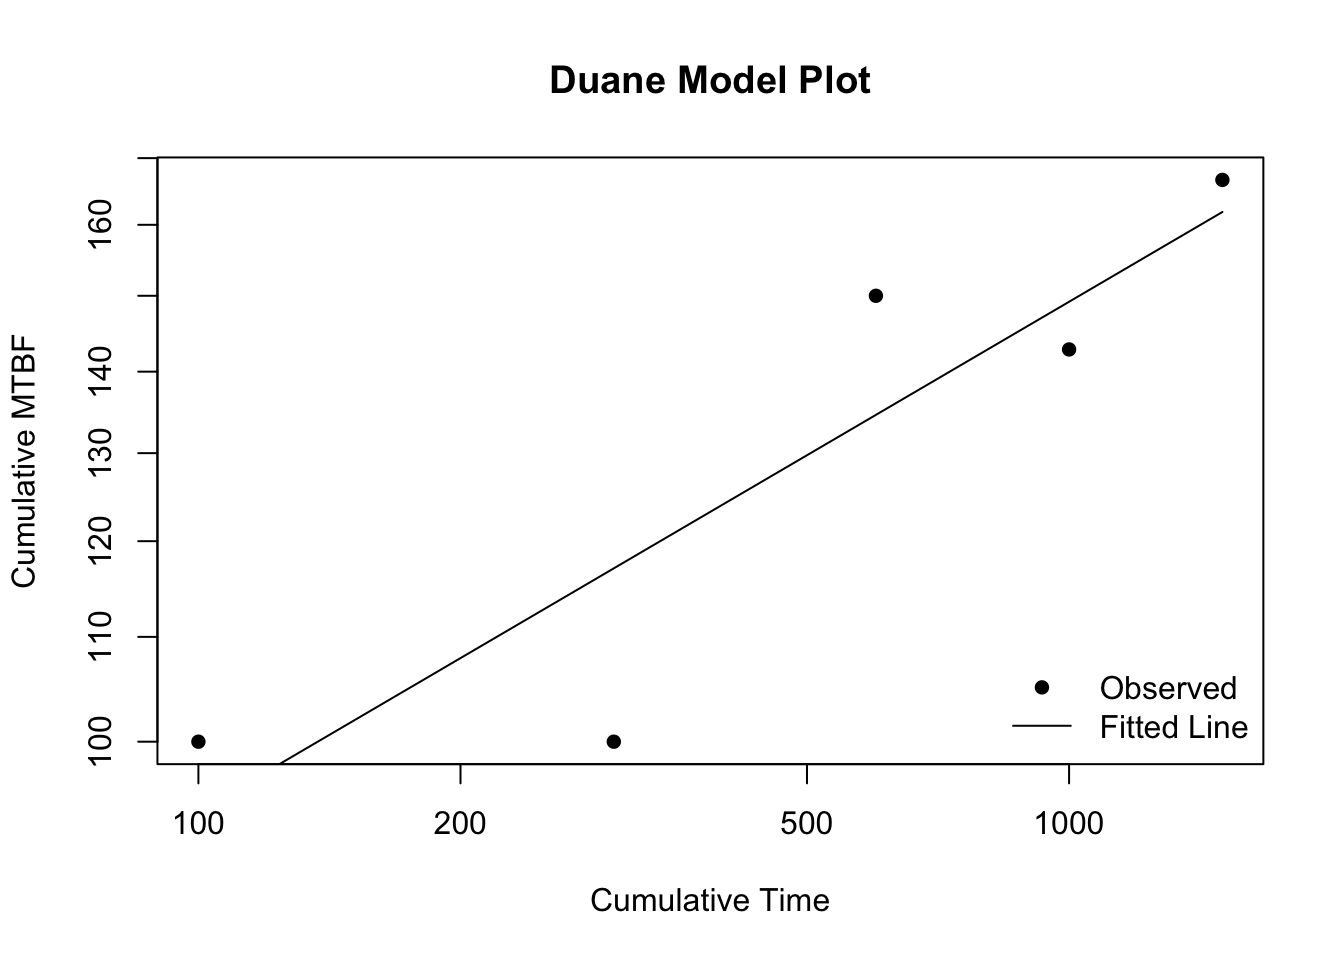
\includegraphics{paper_files/figure-latex/duane-plot-1.pdf}

The plot shows the cumulative MTBF on the y-axis and cumulative time on
the x-axis, with a fitted line indicating the reliability growth trend.
The \texttt{duane\_plot} function returns a \texttt{duane} object with
the model results that can be further customized or saved. To view the
model results, print the \texttt{duane} object using the \texttt{print}
function:

\begin{Shaded}
\begin{Highlighting}[]
\FunctionTok{print}\NormalTok{(fit)}
\end{Highlighting}
\end{Shaded}

\begin{verbatim}
## Duane Analysis Result
## ----------------------
## Linear model (log-log scale): log(MTBF) ~ log(Time)
## 
## Coefficients:
##  (Intercept) log_cum_time 
##    3.6144974    0.2013244 
## 
## AIC: -3.55, BIC: -4.72
\end{verbatim}

\subsubsection{The Crow-AMSAA Model}\label{the-crow-amsaa-model}

The Army Materiel Systems Analysis Activity Model by Crow (Crow-AMSAA)
takes failure behavior as a Non-Homogeneous Poisson Process (NHPP)
governed by a power law, making the model particularly effective for
systems undergoing reliability growth due to continuous improvements.

Similar to the Duane Model, the shape of the model indicates the rate of
reliability growth:

\begin{itemize}
\tightlist
\item
  A model fit with downward curvature means that the system is improving
  (reliability is growing, the failure rate is decreasing).
\item
  A linear model means there is no change in reliability (the system is
  stable).
\item
  A model fit with upward curvature indicates that reliability is
  worsening (the failure rate is increasing).
\end{itemize}

To use the Crow-AMSAA Model in ReliaGrowR, use the \texttt{rga}
function. This function takes a vector of failure times and a vector of
failure counts, and generates a plot of cumulative MTBF vs cumulative
time with the fitted model.

First, set up some dummy cumulative time and failure data:

\begin{Shaded}
\begin{Highlighting}[]
\NormalTok{times }\OtherTok{\textless{}{-}} \FunctionTok{c}\NormalTok{(}\DecValTok{100}\NormalTok{, }\DecValTok{200}\NormalTok{, }\DecValTok{300}\NormalTok{, }\DecValTok{400}\NormalTok{, }\DecValTok{500}\NormalTok{)}
\NormalTok{failures }\OtherTok{\textless{}{-}} \FunctionTok{c}\NormalTok{(}\DecValTok{1}\NormalTok{, }\DecValTok{2}\NormalTok{, }\DecValTok{1}\NormalTok{, }\DecValTok{3}\NormalTok{, }\DecValTok{2}\NormalTok{)}
\end{Highlighting}
\end{Shaded}

Then use the \texttt{rga} function to fit the model and the
\texttt{plot\_rga} function to plot the results:

\begin{Shaded}
\begin{Highlighting}[]
\NormalTok{result }\OtherTok{\textless{}{-}} \FunctionTok{rga}\NormalTok{(times, failures)}
\FunctionTok{plot\_rga}\NormalTok{(result)}
\end{Highlighting}
\end{Shaded}


\includegraphics{paper_files/figure-latex/unnamed-chunk-4-1.pdf}

The \texttt{plot\_rga} function generates a plot showing the cumulative
MTBF on the y-axis and cumulative time on the x-axis, with a fitted
curve indicating the reliability growth trend. The \texttt{rga} function
returns an \texttt{rga} object containing the fitted model parameters.
To view the model results, print the \texttt{rga} object:

\begin{Shaded}
\begin{Highlighting}[]
\FunctionTok{print}\NormalTok{(result)}
\end{Highlighting}
\end{Shaded}

\begin{verbatim}
## Reliability Growth Analysis (RGA)
## ---------------------------------
## Model Type: Crow-AMSAA 
## 
## Parameters (per segment):
##   Beta: 0.7987
##   Lambda: 0.0269
## 
## Goodness of Fit:
##   AIC: -3.55
##   BIC: -4.72
\end{verbatim}

\subsubsection{The Piecewise NHPP Model}\label{the-piecewise-nhpp-model}

The Piecewise NHPP model is an extension of the standard NHPP model that
includes different segments or phases of time that follow separate
failure distributions. This model is particularly useful when a system
experiences changes in failure behavior over different development
phases, such as the initial, interim and final phases of a development
process.

To use the Piecewise NHPP model in ReliaGrowR, first, set up some
cumulative time and failure data and specify a breakpoint:

\begin{Shaded}
\begin{Highlighting}[]
\NormalTok{times }\OtherTok{\textless{}{-}} \FunctionTok{c}\NormalTok{(}\DecValTok{25}\NormalTok{, }\DecValTok{55}\NormalTok{, }\DecValTok{97}\NormalTok{, }\DecValTok{146}\NormalTok{, }\DecValTok{201}\NormalTok{, }\DecValTok{268}\NormalTok{, }\DecValTok{341}\NormalTok{, }\DecValTok{423}\NormalTok{, }\DecValTok{513}\NormalTok{, }\DecValTok{609}\NormalTok{, }\DecValTok{710}\NormalTok{, }\DecValTok{820}\NormalTok{, }\DecValTok{940}\NormalTok{, }\DecValTok{1072}\NormalTok{, }\DecValTok{1217}\NormalTok{)}
\NormalTok{failures }\OtherTok{\textless{}{-}} \FunctionTok{c}\NormalTok{(}\DecValTok{1}\NormalTok{, }\DecValTok{1}\NormalTok{, }\DecValTok{2}\NormalTok{, }\DecValTok{4}\NormalTok{, }\DecValTok{4}\NormalTok{, }\DecValTok{1}\NormalTok{, }\DecValTok{1}\NormalTok{, }\DecValTok{2}\NormalTok{, }\DecValTok{1}\NormalTok{, }\DecValTok{4}\NormalTok{, }\DecValTok{1}\NormalTok{, }\DecValTok{1}\NormalTok{, }\DecValTok{3}\NormalTok{, }\DecValTok{3}\NormalTok{, }\DecValTok{4}\NormalTok{)}
\NormalTok{breaks }\OtherTok{\textless{}{-}} \DecValTok{500}
\end{Highlighting}
\end{Shaded}

Then use the \texttt{rga} function with model type ``Piecewise NHPP
model'' to fit the model and the \texttt{plot\_rga} function to plot the
results:

\begin{Shaded}
\begin{Highlighting}[]
\NormalTok{result }\OtherTok{\textless{}{-}} \FunctionTok{rga}\NormalTok{(times, failures, }\AttributeTok{model\_type =} \StringTok{"Piecewise NHPP"}\NormalTok{, }\AttributeTok{breaks =}\NormalTok{ breaks)}
\FunctionTok{plot\_rga}\NormalTok{(result)}
\end{Highlighting}
\end{Shaded}

\includegraphics{paper_files/figure-latex/unnamed-chunk-7-1.pdf}

To view the model results, print the \texttt{rga} object using the
\texttt{print} function:

\begin{Shaded}
\begin{Highlighting}[]
\FunctionTok{print}\NormalTok{(result)}
\end{Highlighting}
\end{Shaded}

\begin{verbatim}
## Reliability Growth Analysis (RGA)
## ---------------------------------
## Model Type: Piecewise NHPP 
## 
## Breakpoints (original scale):
## 500 
## 
## Parameters (per segment):
##   Betas: 0.8182, 0.3902
##   Lambdas: 0.0642, 0.9362
## 
## Goodness of Fit:
##   AIC: -24.64
##   BIC: -21.10
\end{verbatim}

\subsubsection{The Piecewise NHPP with Change Point
Detection}\label{the-piecewise-nhpp-with-change-point-detection}

The Piecewise NHPP with Change Point Detection is an advanced model to
identify changes in failure behavior and model system reliability. This
method builds on the Piecewise NHPP model by introducing the concept of
change points, which represent the time when the underlying failure
behavior changes. Detection of change points involves statistical
techniques that analyze failure data to automatically identify when the
behavior changes, allowing for a more precise segmentation of the model
into different distributions.

To use the Piecewise NHPP with Change Point Detection in ReliaGrowR, use
the \texttt{rga} function with the model type set to ``Piecewise NHPP''
and breaks set to NULL. The function will automatically detect change
points based on the provided failure data. First, set up some cumulative
time and failure data:

\begin{Shaded}
\begin{Highlighting}[]
\NormalTok{times }\OtherTok{\textless{}{-}} \FunctionTok{c}\NormalTok{(}\DecValTok{25}\NormalTok{, }\DecValTok{55}\NormalTok{, }\DecValTok{97}\NormalTok{, }\DecValTok{146}\NormalTok{, }\DecValTok{201}\NormalTok{, }\DecValTok{268}\NormalTok{, }\DecValTok{341}\NormalTok{, }\DecValTok{423}\NormalTok{, }\DecValTok{513}\NormalTok{, }\DecValTok{609}\NormalTok{, }\DecValTok{710}\NormalTok{, }\DecValTok{820}\NormalTok{, }\DecValTok{940}\NormalTok{, }\DecValTok{1072}\NormalTok{, }\DecValTok{1217}\NormalTok{)}
\NormalTok{failures }\OtherTok{\textless{}{-}} \FunctionTok{c}\NormalTok{(}\DecValTok{1}\NormalTok{, }\DecValTok{1}\NormalTok{, }\DecValTok{2}\NormalTok{, }\DecValTok{4}\NormalTok{, }\DecValTok{4}\NormalTok{, }\DecValTok{1}\NormalTok{, }\DecValTok{1}\NormalTok{, }\DecValTok{2}\NormalTok{, }\DecValTok{1}\NormalTok{, }\DecValTok{4}\NormalTok{, }\DecValTok{1}\NormalTok{, }\DecValTok{1}\NormalTok{, }\DecValTok{3}\NormalTok{, }\DecValTok{3}\NormalTok{, }\DecValTok{4}\NormalTok{)}
\end{Highlighting}
\end{Shaded}

Then use the \texttt{rga} function with model type ``Piecewise NHPP
model'' to fit the model and the \texttt{plot\_rga} function to plot the
results:

\begin{Shaded}
\begin{Highlighting}[]
\NormalTok{result }\OtherTok{\textless{}{-}} \FunctionTok{rga}\NormalTok{(times, failures, }\AttributeTok{model\_type =} \StringTok{"Piecewise NHPP"}\NormalTok{)}
\FunctionTok{plot\_rga}\NormalTok{(result)}
\end{Highlighting}
\end{Shaded}


\includegraphics{paper_files/figure-latex/unnamed-chunk-10-1.pdf}

Print the \texttt{rga} object using the \texttt{print} function to view
the model results:

\begin{Shaded}
\begin{Highlighting}[]
\FunctionTok{print}\NormalTok{(result)}
\end{Highlighting}
\end{Shaded}

\begin{verbatim}
## Reliability Growth Analysis (RGA)
## ---------------------------------
## Model Type: Piecewise NHPP 
## 
## Breakpoints (original scale):
## 523.9797 
## 
## Parameters (per segment):
##   Betas: 0.8182, 0.3902
##   Lambdas: 0.0642, 0.9362
## 
## Goodness of Fit:
##   AIC: -24.64
##   BIC: -21.10
\end{verbatim}

\subsection{Verification}\label{verification}

ReliaGrowR was verified through unit tests and example analyses to
ensure that the package performs as expected. The package includes a
suite of tests that cover the core functionalities, including model
fitting, plotting, and change point detection. These tests run
automatically during package development to ensure reliability and
correctness.

ReliaGrowR was also tested on different operating systems and R versions
to ensure compatibility and performance. The results of these tests are
documented on CRAN. Full documentation and working examples are
available on the project website, where users can also contribute to or
report issues with the package.

\subsection{Extensibility}\label{extensibility}

ReliaGrowR is designed to be extensible, allowing users to add custom
models or features as needed. The package has already been extended in
several ways, including education {[}11{]}, advanced visualization
{[}12{]}, and web-based applications {[}13{]}. The package is
experimental and is in active development with new features and models
being added regularly. Users can contribute to the package by submitting
pull requests on the project repository, where the source code is
hosted. The package is also open to contributions from the community,
and users are encouraged to report issues or suggest improvements.

\subsection{References}\label{references}

\begin{enumerate}
\def\labelenumi{\arabic{enumi}.}
\item
  Placeholder, ``ReliaGrowR: Reliability Growth Analysis'', R package
  version 0.1, 2024, \url{doi:10.32614/CRAN.package.ReliaGrowR},
  \url{https://cran.r-project.org/package=ReliaGrowR}.
\item
  R Core Team, ``R: A Language and Environment for Statistical
  Computing'', R Foundation for Statistical Computing, Vienna, Austria,
  2024, \url{https://www.R-project.org/}.
\item
  D. Silkworth, J. Symynck, ``WeibullR: Weibull Analysis for Reliability
  Engineering'', R package version 1.2.1, 2022,
  \url{https://CRAN.R-project.org/package=WeibullR}.
\item
  D. Silkworth, ``WeibullR.ALT: Accelerated Life Testing Using
  `WeibullR'\,'', R package version 0.7.2, 2022,
  \url{https://CRAN.R-project.org/package=WeibullR.ALT}.
\item
  M. Reid, ``Reliability -- a Python library for reliability
  engineering'', Version 0.8.2, 2022,
  \url{https://doi.org/10.5281/ZENODO.3938000}.
\item
  J. T. Duane, ``Learning Curve Approach to Reliability Monitoring'',
  IEEE Transactions on Aerospace, vol.~2, no. 2, pp.~563-566, April
  1964, doi: 10.1109/TA.1964.4319640.
\item
  L.H. Crow, ``Reliability analysis for complex repairable systems.'',
  Reliability and biometry: Statistical analysis of lifelength,
  pp.~379-410, 1974.
\item
  H. Guo, A. Mettas, G. Sarakakis and P. Niu, ``Piecewise NHPP models
  with maximum likelihood estimation for repairable systems'', 2010
  Proceedings - Annual Reliability and Maintainability Symposium (RAMS),
  San Jose, CA, USA, 2010, pp.~1-7, \url{doi:10.1109/RAMS.2010.5448029}.
\item
  S. Fasola, V.M.R Muggeo, K. Kuchenhoff, ``A heuristic, iterative
  algorithm for change-point detection in abrupt change models'',
  Computational Statistics, 33, pp.~997-1015, 2018.
\item
  V.M.V Muggeo, ``segmented: an R Package to Fit Regression Models with
  Broken-Line Relationships'', R News, 8/1, pp.~20-25,
  \url{https://cran.r-project.org/doc/Rnews/}.
\item
  Placeholder, ``WeibullR.learnr: An Interactive Introduction to Life
  Data Analysis'', R package version 0.1.1, 2023,
  \url{doi:10.32614/CRAN.package.WeibullR.learnr},
  \url{https://CRAN.R-project.org/package=WeibullR.learnr}.
\item
  Placeholder, ``WeibullR.plotly: Interactive Weibull Probability
  Plots'', R package version 0.2.0, 2023,
  \url{doi:10.32614/CRAN.package.WeibullR.plotly}
  \url{https://CRAN.R-project.org/package=WeibullR.plotly}.
\item
  Placeholder, ``WeibullR.shiny: A Shiny App for Weibull Analysis'', R
  package version 0.2.0, 2023,
  \url{doi:10.32614/CRAN.package.WeibullR.shiny}
  \url{https://CRAN.R-project.org/package=WeibullR.shiny}.
\end{enumerate}

\end{document}
